% Drawing 148/02-19 -- folder 148, batch 02, archive page 35 (PDF page 36).
% Transcription: au bas de la page, un petit croquis au crayon : un triangle entouré d'un ovale, des pointes de flèche sur deux de ses côtés, un petit anneau près du sommet du haut et un chiffre au centre.
% Kind: small pencil triangle in an oval. Method 2 (schematic redraw from the facsimile). Status: partial.
% Notes: Faint pencil and ink. A tetrahedron seen from above, not a plain triangle: the apex, the three edges from it to a left, a front and a right vertex, and below them the edge from the left vertex to the front one (gone over, with an arrowhead pointing to the front vertex at about two thirds of its length and a short separate stroke at its left end); the hidden edge from the left vertex to the right one is drawn only in its left third and in its last few units, where it ends with a lower barb in an arrowhead at the right vertex. A ring round the apex cuts the three edges just below it. A pencil loop starting in a small hook at the upper left runs round the left vertex and under the figure; a short faint stroke stands at the right of the right edge. Left out: the small open curl at the centre (an open loop with a tick, in browner ink), which the transcription reads as a digit; it is not legible as one (3, 9 or a turning sign). Redrawn 2026-11-12 (issue 128). 2026-11-13, Claude Opus 5.5, issue 147, overlay check: not compiled (no TeX in the session); the TikZ was rasterised by a local interpreter and laid over the 236 ppi scan rendered at 400 dpi. Redrawn on the ink: each stroke fitted on its ink (straight strokes by least squares, the loop and the front edge through points moved onto their ink); every stroke lies on its ink to within about half a unit. Changed: the figure is a tetrahedron with four vertices, not a triangle with an oval round its lower part: the earlier redraw had the oval centred on the triangle and the arrowheads on the wrong strokes. Still differs: only the sign at the centre, left out as unread. Disagreement with the transcription: « un triangle » is a tetrahedron (three edges from the apex, a front edge, a partly drawn hidden edge); the oval is an open loop round the left vertex, not round the triangle.
% Coordinates: 1 unit = 1 mm = 1/100 of the crop width, y downwards as on the crop (bbox in page fractions: [0.49, 0.765, 0.63, 0.84]).
% Redrawn by Claude (claude-fable-5-2), issue #128, 2026-11-12; not checked by a human; not compiled (no TeX in the session); overlay-checked on the scan by Claude Opus 5.5, issue #147, 2026-11-13, not compiled (no TeX in the session).
% Rights: reproduces part of the work -- behind RENDER_TRANSCRIPTS, never published by itself.
\documentclass[tikz,border=3pt]{standalone}
\usepackage{amsmath,amssymb}
\usetikzlibrary{patterns,arrows.meta}
\tikzset{pencil/.style={black!45}, struck/.style={black!35}, mpt/.style={circle,draw,inner sep=1.3pt}, pt/.style={circle,fill,inner sep=0.9pt}, opt/.style={circle,draw,fill=white,inner sep=1.1pt}, Rd/.style={red!75!black}, Gn/.style={green!45!black}, Br/.style={brown!70!black}}
\begin{document}
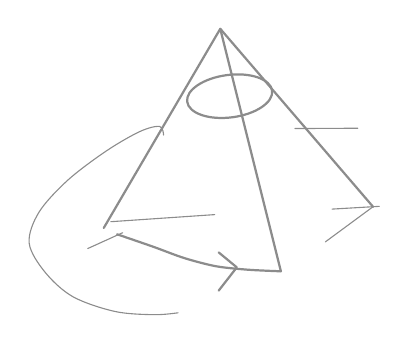
\begin{tikzpicture}[x=1mm,y=-1mm,line cap=round,line join=round,font=\small]
\coordinate (T) at (51.4,26.8);
\coordinate (L) at (36.6,52.1);
\coordinate (F) at (59.1,57.6);
\coordinate (R) at (70.8,49.4);
% the three edges from the apex
\draw[pencil,thick] (L) -- (T) -- (F);
\draw[pencil,thick] (T) -- (R);
% the hidden edge, from the left vertex (the middle of it not drawn on the page), ending in the arrowhead at the right vertex
\draw[pencil] (37.5,51.3) -- (50.7,50.4);
\draw[pencil] (65.6,49.7) -- (71.6,49.35);
\draw[pencil] (64.75,53.86) -- (R);
% the front edge, a short stroke at the left, and its arrowhead
\draw[pencil] (34.57,54.71) -- (39,52.7);
\draw[pencil,thick] plot[smooth, tension=0.5] coordinates {(38.3,52.9) (42.91,54.49) (46.86,55.93) (50.87,56.96) (54.94,57.4) (F)};
\draw[pencil,thick] (51.2,55.2) -- (53.5,57.1) -- (51.2,60.05);
% ring round the apex
\draw[pencil,thick,rotate around={7.4:(52.59,35.36)}] (52.59,35.36) ellipse [x radius=5.44, y radius=2.7];
% the loop round the lower left, starting in a small hook
\draw[pencil] plot[smooth, tension=0.55] coordinates {(44.2,40.3) (43.7,39.2) (41.21,39.84) (36.95,42.3) (32.03,46.03) (28.38,50.09) (27.13,54.01) (29.16,57.73) (32.69,60.83) (38.02,62.7) (43,63.11) (46.04,62.87)};
\draw[pencil] (60.89,39.47) -- (68.88,39.43);
\end{tikzpicture}
\end{document}
